\documentclass[a4paper,twoside]{article}

\usepackage{epsfig}
\usepackage{subfigure}
\usepackage{calc}
\usepackage{amssymb}
\usepackage{amstext}
\usepackage{amsmath}
\usepackage{amsthm}
\usepackage{multicol}
\usepackage{pslatex}
\usepackage{apalike}

%%%% Template Packages %%%%

%\usepackage[usenames]{color}
%\usepackage{xcolor}
%\usepackage{makeidx}
%\usepackage{graphicx}
%\usepackage{epsfig}
%\usepackage{xspace}
%\usepackage{pstricks}
%\usepackage{pst-node}
%\usepackage{pst-tree}
%\usepackage{pst-plot}
%\usepackage[nonumberlist, toc, style=super]{glossaries}
\usepackage[colorlinks]{hyperref}
%\usepackage{zed-csp}
%\usepackage{psfrag}
%\usepackage{ae}
%\usepackage{txfonts}
%\usepackage{ifthen}  
%\usepackage{alltt}
%\usepackage{url} 
%\usepackage{epsfig}
%\usepackage{listings}
%\usepackage{color,listings}
%\usepackage{rotating}
%\usepackage{longtable}
%\usepackage{fancyhdr}
%\usepackage[colorinlistoftodos]{todonotes}
%\usepackage{multirow}
%\usepackage{subfig}
%\usepackage{tabularx}
%\usepackage{array}
\usepackage[utf8]{inputenc}
%\usepackage{acronym}
\usepackage{setspace}

%\usepackage{titlesec}


%\usepackage{graphicx} % Required to insert images
%\usepackage{float}
%\usepackage{listings}

\usepackage{amsmath}
\usepackage{amsthm}
\usepackage{amssymb}

\usepackage{natbib}
\usepackage[nottoc,notlot,notlof]{tocbibind}

\usepackage{tikz}
\usetikzlibrary{backgrounds}
\usetikzlibrary{arrows}

\usepackage{algorithm}
\usepackage{algpseudocode}
\usepackage{algorithmicx}

\usepackage{subcaption}

\usepackage{SCITEPRESS}     % Please add other packages that you may need BEFORE the SCITEPRESS.sty package.

%%%%%%%%%%%%%% GENERAL %%%%%%%%%%%%%%
\newcommand{\ct}{\sim}

\newcommand{\ms}[1]{\overset{#1}{\leftarrow}}
\newcommand{\mt}[1]{\overset{#1}{\rightarrow}}

%%%%%%%%%%%%%% GG %%%%%%%%%%%%%%
\newcommand{\neigh}[1]{\operatorname{neigh}_{#1}}
\newcommand{\isomorph}{\cong}
\newcommand{\scont}[2]{\eta_{#1}(#2)}
\newcommand{\cont}[2]{\operatorname{cont}_{#1}(#2)}
\newcommand{\emb}[1]{\operatorname{emb}(#1)}
\newcommand{\allgraphs}[1]{\mathcal{G}_{#1}}
\newcommand{\startG}[1]{Z_{#1}}
\newcommand{\pro}{\to}

%%%%%%%%%%%%%% TGG %%%%%%%%%%%%%%
\newcommand{\alltgraphs}[1]{\mathcal{TG}_{#1}}
\newcommand{\startTG}[1]{Z_{#1}}
\newcommand{\emptyTG}{\varepsilon}
\newcommand{\source}{\operatorname{s}}
\newcommand{\Source}{\operatorname{S}}
\newcommand{\target}{\operatorname{t}}
\newcommand{\Target}{\operatorname{T}}
\newcommand{\cderiv}[3]{
	\ifx\relax#2\relax%
	\overset{#1}{\Rrightarrow}_{#3}%
	\else
	\overset{#1,#2}{\Rrightarrow}_{#3}%
	\fi
}
\newcommand{\deriv}[3]{
	\ifx\relax#2\relax
	\overset{#1}{\Rightarrow}_{#3}
	\else
	\overset{#1,#2}{\Rightarrow}_{#3}
	\fi
}
\newcommand{\derivtr}[1]{
	\Rightarrow^*_{#1}
}
\newcommand{\tcderiv}[3]{
	\ifx\relax#2\relax
	\overset{#1}{\Rrightarrow}_{#3}
	\else
	\overset{#1,#2}{\Rrightarrow}_{#3}
	\fi
}
\newcommand{\tderiv}[3]{
	\ifx\relax#2\relax
	\overset{#1}{\Rightarrow}_{#3}
	\else
	\overset{#1,#2}{\Rightarrow}_{#3}
	\fi
}
\newcommand{\tderivtr}[1]{\Rightarrow^*_{#1}}

%%%% PAC %%%%
\newcommand{\cderivpac}[4]{\overset{#1,#2,#3}{\Rrightarrow}_{#4}}
\newcommand{\derivpac}[4]{
	\ifx\relax#3\relax
	\overset{#1,#2}{\Rightarrow}_{#4}
	\else
	\overset{#1,#2,#3}{\Rightarrow}_{#4}
	\fi}
\newcommand{\derivpacn}[2]{\Rightarrow^{#2}_{#1}}
\newcommand{\resolv}[1]{\overset{#1}{\rightarrowtail}}
\newcommand{\resolvn}[2]{\overset{#1}{\rightarrowtail}^{#2}}
\newcommand{\derivpactr}[1]{\Rightarrow^*_{#1}}
\newcommand{\resolvtr}[1]{\rightarrowtail^*}

\newcommand{\tcderivpac}[4]{\overset{#1,#2,#3}{\Rrightarrow}_{#4}}
\newcommand{\tderivpac}[4]{
	\ifx\relax#3\relax
	\overset{#1,#2}{\Rightarrow}_{#4}
	\else
	\overset{#1,#2,#3}{\Rightarrow}_{#4}
	\fi
}
\newcommand{\tderivpacn}[2]{\Rightarrow^{#2}_{#1}}
\newcommand{\tresolv}[1]{\overset{#1}{\rightarrowtail}}
\newcommand{\tresolvn}[2]{\overset{#1}{\rightarrowtail}^{#2}}
\newcommand{\tderivpactr}[1]{\Rightarrow^*_{#1}}
\newcommand{\tresolvtr}[1]{\rightarrowtail^*_{#1}}



%%%%%%%%%%%%%% TIKZ %%%%%%%%%%%%%%
\tikzstyle{grammar}=[shorten >= 1pt, ->, draw=black!50, framed, background rectangle/.style={draw, rounded corners}, font=\scriptsize ]
\tikzstyle{graph}=[shorten >= 1pt, ->, draw=black!50, font=\scriptsize]
\tikzstyle{rid} = [inner sep=3pt, align=left, anchor=east]
\tikzstyle{nont}=[rectangle, inner sep=3pt, draw, fill=white, minimum width=5pt]
\tikzstyle{t}=[circle, inner sep=1pt, draw, fill=white, minimum width=5pt]
\tikzstyle{pac}=[circle, inner sep=1pt, draw, dotted, fill=white, minimum width=5pt]
\tikzstyle{empty}=[font=\Large, fill=white]
\tikzstyle{g}=[inner sep=3pt, fill=white]
\tikzstyle{lhs}=[inner sep=1pt, fill=white]
\tikzstyle{w}=[circle, inner sep=1pt, below=8pt, draw, fill=white, font=\tiny]
\tikzstyle{uw}=[circle, inner sep=1pt, above=8pt, draw, fill=white, font=\tiny]
\tikzstyle{edge}=[->, thin, -latex]
\tikzstyle{pacedge}=[->, thin, -latex, dotted]
\tikzstyle{edgeLabel}=[midway, above]
\tikzstyle{vledgeLabel}=[midway, left]
\tikzstyle{vredgeLabel}=[midway, right]
\tikzstyle{vbedgeLabel}=[above=3pt]
\tikzstyle{wedge}=[-, thin]
\tikzstyle{biedge}=[-, thin]
\tikzstyle{pipe}=[-, thick]
\tikzstyle{morph}=[-, thin, dashed, -latex]

\newcommand{\ridX}{-0.3}
\newcommand{\ridY}{0.5}
\newcommand{\lhsX}{-0.3}
\newcommand{\pipeUY}{-0.5}
\newcommand{\pipeBY}{0.5}

%% Scheme %%
\tikzstyle{scheme}=[shorten >= 1pt, ->, draw=black!50, framed, background rectangle/.style={draw, rounded corners}, font=\scriptsize ]
\tikzstyle{object}=[rectangle, inner sep=3pt, draw, fill=white, minimum width=5pt]
\tikzstyle{metaobject}=[rectangle, inner sep=3pt, draw, dashed, fill=white, minimum width=5pt]
\tikzstyle{activity}=[rectangle, inner sep=3pt, draw, fill=white, minimum width=5pt, rounded corners]

\subfigtopskip=0pt
\subfigcapskip=0pt
\subfigbottomskip=0pt

\begin{document}

\title{Model Transformation with Context-free Triple Graph Grammars and Application Conditions}

%\author{\authorname{William da Silva\sup{1,2}, Max Bureck\sup{1} and Ina Schieferdecker\sup{1,2} and Christian Hein\sup{1}}
%\affiliation{\sup{1}Fraunhofer Fokus Institute, Berlin, Germany}
%\affiliation{\sup{2}Technische Universität Berlin, Berlin, Germany}
%\email{\{william.bombardelli.da.silva, max.bureck\}@fokus.fraunhofer.de}
%}

\keywords{Triple Graph Grammars, NCE Graph Grammars, Model Transformation, Model-driven Development.}

%TODO: Between 70 and 200 words
\abstract{}

\onecolumn \maketitle \normalsize \vfill

%TODO: Decide on the use of italic
%TODO: Decide whether ms or m_s mt or m_t?
%TODO: Number the definitions and examples
\section{\uppercase{Introduction}}

\noindent Model transformation is a very important topic for the Model-driven Development (MDD) approach. In special, the problem of specifying model transformation between two metamodels is very significant for the application of MDD in practice. In this regard, the rule-based approach with triple graph grammars (TGG) proposes a technique to describe model transformation by means of a context-sensitive grammar of triple graphs.

%TODO: Maybe add reference to TGG
A triple graph $G_s \ms{ms} G_c \mt{mt} G_t$ consists of three disjunct labeled graphs $G_s$, $G_c$, $G_t$, called source, correspondence, and target graphs, respectively, where the $G_s$ and $G_t$ contain elements of the two metamodels being specified, and $G_c$ contains elements that connect $G_s$ and $G_t$ via two partial mappings $ms: G_c \pto G_s$ and $mt: G_c \pto G_t$ \cite{schurr1994specification}. A triple graph can therefore express connections between elements of two metamodels (the source and the target), what in turn can be used to specify which elements of the source side is to be transformed into which elements of the target side. To accomplish that, triple graphs are combined in a triple graph grammar.

A TGG consists of a set of rules of the form $L \pro R$, where $L$ and $R$ are triple graphs and $L$ is contained in $R$ ($L \subset R$). Therewith, each rule describes one unit of the transformation between the source and target metamodels referred by $L$ and $R$. The application of a rule $L \pro R$ on a triple graph $G$ can be informally understood as the removal of the occurrence of $L$ in $G$ by $R$. By this means, a TGG, analogously to common string grammars, characterizes a language of triple graphs, that consists of all triple graphs generated by consecutive rules applications starting from a special initial triple graph $Z_G$.

Such TGG specifications are often required to be correct, easy to construct and comprehensible not only by the author. Thereby, the grammar size (i.e. the number of rules and elements in the rules) and the possibility to express abstract concepts with the rules become crucial requirements for a TGG formalism. We have identified that for some transformations these requirements are not optimally fulfilled by the current state-of-the-art of the TGG formalism. In particular, the standard version of TGG does not admit the expression of abstract notions like inheritance, what leads to grammars with bigger sizes and that are more difficult to comprehend.

In order to solve this problem, we propose in this paper a modified version of the TGG formalism that introduces the concept of non-terminal symbols and that requires the grammar rules to be context-free, that is of the from $A \pro R$, where $A$ is only one symbol and $R$ a triple graph. Moreover, we also include in our formalism an application condition mechanism that should enhance its expressiveness and usability. Our proposal is inspired by the use non-terminal symbols in string grammars, that allows the creation of simpler grammars for which there are more efficient recognizer algorithms and with which it has become possible to built efficient programming language compilers.

Our new TGG formalism is strongly based on the results of \cite{rozenberg1986boundary} and \cite{janssens1982graph} for graph grammars with non-terminal symbols, called \textit{graph grammars with neighborhood-controlled embedding} (NCE graph grammars) . What we present in this paper is basically the transportation of the advances of NCE graph grammars to TGG, and extend it with a positive application condition mechanism. We name this new version of TGG as NCE TGG.

%TODO: Check table with results 
Our results include the presentation of the NCE TGG as well as of a parsing and transformation procedure suitable for batch bidirectional transformation and an experimental evaluation that evinces the potential of our proposal. In fact, with NCE TGG we could specify one transformation that we could not with the standard TGG, and from other four evaluated use cases, NCE TGG outperformed standard TGG in one scenario. Moreover, we claim that the cognitive effort to comprehend a NCE TGG is lesser in comparison with TGG, by its context-free characteristic and, thus, proximity with other popular grammar formalisms for computer scientists, like the LL and LR grammars of high-level programming language compilers.

%TODO: Remainder
The remainder of this paper is as follows...

\section{\uppercase{Related Works}}

\noindent In this section, we offer a short literary review on the graph grammar and triple graph grammar approaches that are more relevant to our work. We focus, therefore, on the context-free node label replacement approach for graph grammars, although, there is a myriad of different alternatives to it, for example, the algebraic approach \cite{ehrig1999handbook}. We refer to context-free grammars, inspired by the use of such classification for string grammars, in a relaxed way without any compromise to any definition.

In the node label replacement context-free formalisms stand out the \textit{node label controlled graph grammar} (NLC) and its successor \textit{graph grammar with neighborhood-controlled embedding} (NCE). NLC is based on the replacement of one vertex by a graph, governed by embedding rules written in terms of the vertex's label \cite{rozenberg1986boundary}. For various classes of these grammars, there exist polynomial-time top-down and bottom-up parsing algorithms \cite{flasinski1993parsing,flasinski2014characteristics,rozenberg1986boundary,wanke1991algorithms}. The recognition complexity and generation power of such grammars have also been analyzed \cite{flasinski1998power,kim2012structure}. NCE occurs in several formulations, including a context-sensitive one, but here we focus on the context-free formulation, where one vertex is replaced by a graph, and the embedding rules are written in terms of the vertex's neighbors \cite{janssens1982graph,skodinis1998neighborhood}. For some classes of these grammars, polynomial-time bottom-up parsing algorithms and automaton formalisms were proposed and analyzed \cite{kim2001efficient,brandenburg2005finite}. In special, one of these classes is the \textit{boundary graph grammar with neighborhood-controlled embedding} (BNCE), that is used in our approach for model transformation.

Regarding TGG \cite{schurr1994specification}, a 20 years review of the realm is put forward by Anjorin et al. \cite{anjorin201620}. In special, advances are made in the direction of expressiveness with the introduction of application conditions \cite{klar2010extended} and of modularization \cite{anjorin2014modularizing}. Furthermore, in the algebraic approach for graph grammars, we have found proposals that introduce inheritance \cite{bardohl2004integrating,hermann2008typed} and variables \cite{hoffmann2005graph} to the formalisms. Nevertheless, we do not know any approach that introduces non-terminal symbols to TGG with the purpose of gaining expressiveness or usability. In this sense, our proposal brings something new to the current state-of-the-art.

\section{\uppercase{Context-free TGG}}

\noindent In this section, we present our main contribution, that is the application of the ideas of NCE graph grammars from \cite{rozenberg1986boundary} and \cite{janssens1982graph} to the creation of a context-free version of TGG with a positive application condition (PAC NCE TGG). For that end, consider first some preliminary definitions.

\begin{definition}
	\label{def:graph}
	A directed labeled graph $G$ over the finite set of symbols $\Sigma$, $G = (V, E, \phi)$ consists of a finite set of vertices $V$, a set of labeled directed edges $E \subseteq V \times \Sigma \times V$ and a total vertex labeling function $\phi : V \to \Sigma$. 
\end{definition}

We refer to directed labeled graphs often referred simply as graphs. For a fixed graph $G$ we refer to its components as $V_G$, $E_G$ and $\phi_G$. Two graphs $G$ and $H$ are disjoint if, and only if, $V_G \cap V_H = \emptyset$. In special, we do not allow loops (vertices of the form $(v,l,v)$).

\begin{definition}
	An isomorphism of directed labeled graphs $G$ and $H$ is a bijective mapping $m: V_G \to V_H$ that maintains the connections between vertices and their labels, that is, $(v,l,w) \in E_G$ if, and only if, $(m(v),l,m(w)) \in E_H$ and $\phi_G(v) = \phi_H(m(v))$.
\end{definition}

We denote the equivalence class of all graphs isomorphic to $G$ by $[G]$.

\begin{definition}
	A directed labeled triple graph $TG = G_s \ms{m_s} G_c \mt{m_t} G_t$ over $\Sigma$ consists of three disjoint directed labeled graphs over $\Sigma$, respectively, the source graph $G_s$, the correspondence graph $G_c$ and the target graph $G_t$, together with two injective partial morphisms $m_s: V_{G_c} \pto V_{G_s}$ and $m_t : V_{G_c} \pto G_{G_t}$.
\end{definition}

We denote the set of all triple graphs over $\Sigma$ as $\alltgraphs{\Sigma}$ and we define the special empty triple graph as $\emptyTG := E \ms{m_s} E \mt{m_t} E$ with $E = (\emptyset, \emptyset, \emptyset)$ and $m_s = m_t = \emptyset$. Moreover, we refer to directed labeled triple graphs are often simply as triple graphs in this paper and we might omit the morphisms' names in the notation. We also advise that in the literature, triple graphs are often modeled as typed graphs, but we judge that for our circumstance labeled graphs fit better and we are convinced that such divergence does not threaten the validity of our approach.

\begin{definition}
	A triple graph grammar with neighborhood-controlled embedding with positive application conditions (PAC NCE TGG) $TGG = (\Sigma, \Delta \subseteq \Sigma, S \in \Sigma, P)$ consists of an alphabet $\Sigma$, a set of terminal symbols $\Delta$ (also define $\Gamma := \Sigma \setminus \Delta$), a start symbol $S$ and a set of production rules $P$ of the form $(A \pro (R_s \ms{} R_c \mt{} R_t), \omega_s, \omega_t, U_s, U_t)$ with $A \in \Gamma$ being the left-hand side, $(R_s \ms{} R_c \mt{} R_t) \in \alltgraphs{\Sigma}$ the right-hand side and $\omega_s : V_{R_s} \pto 2^{\Sigma \times \Sigma}$ and $\omega_t : V_{R_t} \pto 2^{\Sigma \times \Sigma}$ the partial embedding functions from the right-hand side's vertices to pairs of edge and vertex labels and $U_s \subseteq \{v \in V_{R_s} \st \phi_{R_s}(v) \in \Delta\}$ the set of PAC vertices of $R_s$ and $U_t \subseteq \{v \in V_{R_t} \st \phi_{R_t}(v) \in \Delta\}$ the set of PAC vertices of $R_t$.
\end{definition}

If all rules of a PAC NCE TGG have $U = \emptyset$, then we refer to it simply as NCE TGG. For convenience, we define the start triple graph of $TGG$ as $\startTG{TGG} := Z_s \ms{ms} Z_c \mt{mt} Z_t$ where $Z_s = (\{s_0\},\emptyset,\{s_0 \mapsto S\})$, $Z_c = (\{c_0\},\emptyset,\{c_0 \mapsto S\})$, $Z_t = (\{t_0\},\emptyset,\{t_0 \mapsto S\})$, $ms = \{c_0 \mapsto s_0 \}$ and $mt = \{c_0 \mapsto t_0 \}$.

The application of a grammar rule $r = (A \pro (R_s \ms{} R_c \mt{} R_t), \omega_s, \omega_t, U_s, U_t)$ using vertices $v_s$, $v_c$, and $v_t$ to a triple graph $G$ that produces another triple graph $H$, we write $G \tcderivpac{r}{v_s,v_c,v_t}{U_s,U_t}{TGG} H$, can be informally described as the replacement of a non-terminal vertex $v_s$ with label $A$ and all its adjacent edges in $G_s$ by a graph $R_s$ plus edges $e$ between former neighbors $w$ of $v$ and some vertices $t$ of $R_s$, provided $e$'s label and $w$'s label are in the embedding specification $\omega_s(t)$. That is, the embedding function $\omega_s$ of a rule specifies which neighbors of $v_s$ are to be connected with which vertices of $R_s$, according to their labels and the adjacent edges' labels. The process that governs the creation of these edges is called embedding and can occur in various forms in different graph grammar formalisms. We opted for a rather simple approach, in which the edges' directions and labels are maintained. The same replacement procedure occurs simultaneously for the correspondence and target graph using the vertex $v_c$, $v_t$ and graphs $G_c$, $G_t$, $R_c$ and $R_t$.

The most important difference between the traditional TGG and the NCE TGG is that the former allows any triple graph to occur in the left-hand sides, whereas the latter only one symbol. In addition to that, traditional TGG requires that the whole left-hand side occur also in the right-hand side, that is to say, the rules are monotonic. Therewith, embedding is not an issue, because an occurrence of the left-hand side is not effectively replaced by the right-hand side, instead, only new vertices are added. On the other hand, NCE TGG has to deal with embedding through the embedding function.

%TODO: Maybe say m is a triple isomorphism
If $G \tcderivpac{r}{v_s,v_c,v_t}{U_s,U_t}{TGG} H$ and $H' \in [H]$, then we write $G \tderivpac{r}{v_s,v_c,v_t}{W_s,W_t}{TGG} H'$ and call it a derivation step, where $W_s = m(U_s)$ and $W_t = m(U_t)$ where $m$ is the isomorphism from $H$ and $H'$. We might omit identifiers, when the context let them clear.

In the sequel, we give an example for a NCE TGG that specifies the transformation between two different metamodels, the $Pseudocode$ and $Controlflow$ metamodels, whose models are encoded via $Pseudocode$ and $Controlflow$ graphs, respectively.

\begin{example}
	\label{ex:pseudocode2controlflow}
	A $Pseudocode$ graph is an abstract representation of a program written in a pseudo-code where vertices refer to \textit{actions}, \textit{ifs} or \textit{whiles} and edges connect these items together according to how they appear in the program. A $Controlflow$ graph is a more abstract representation of a program, where vertices can only be either a \textit{command} or a \textit{branch}.
	
	Consider, for instance, the program $main$, written in a pseudo-code, and the triple graph $TG$ in Figure \ref{fig:p2c-tg}. The triple graph $TG$ consists of the $Pseudocode$ graph of $main$ connected to the $Controlflow$ graph of the same program through the correspondence graph in the middle of them. In such graph, the vertex labels of the $Pseudocode$ graph $p, i, a, w$ correspond to the concepts of \textit{program}, \textit{if}, \textit{action} and \textit{while}, respectively. The edge label $f$ is given to the edge from the vertex $p$ to the program's first statement, $x$ stands for \textit{next} and indicates that a statement is followed by another statement, $p$ and $n$ stand for \textit{positive} and \textit{negative} and indicate which assignments correspond to the positive of negative case of the \textit{if}'s evaluation, finally $l$ stands for \textit{last} and indicates the last action of a loop. In the $Controlflow$ graph, the vertex labels $g, b, c$ stand for the concepts of \textit{graph}, \textit{branch} and \textit{command}, respectively. The edge label $r$ is given to the edge from the vertex $g$ to the first program's statement, $x, p$ and $n$ mean, analogous to the former graph, \textit{next}, \textit{positive} and \textit{negative}. In the correspondence graph, the labels $pg, ib, ac, wb$ serve to indicate which labels in the source and target graphs are being connected through the triple graph's morphism.
	%TODO: advise that command are not stuffed with further information that actually characterizes them. But it could be done with a future work on attributed graphs
	
	The main difference between the two graphs is the absence of the $w$ label in the $Controlflow$ graph, what makes it encode loops through the combination of $b$-labeled vertices and $x$-labeled edges.
	
	\begin{figure*}
		\begin{minipage}[h]{.48\textwidth}
	\begin{algorithmic}[!ht]
		\State \Program $main(n)$
		\If {$n < 0$}
			\State \Return $\Nothing$
		\Else
			\State $f \gets 1$ 
			\While {$n > 0$}
				\State $f \gets f * n$
				\State $n \gets n - 1$
			\EndWhile
			\State \Return $\Just f$
		\EndIf
	\end{algorithmic}
\end{minipage}
\begin{minipage}[h]{.5\textwidth}
	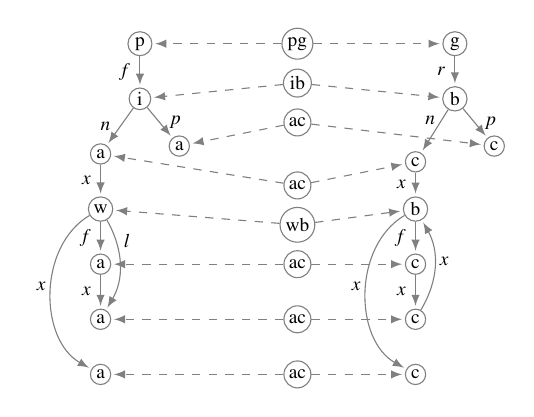
\begin{tikzpicture}[graph]
	\draw (1,0) node[t] (s1) {p};
	\draw (1,-0.7) node[t] (s2) {i};
	\draw (1.5,-1.3) node[t] (s3) {a};
	\draw (0.5,-1.4) node[t] (s4) {a};
	\draw (0.5,-2.1) node[t] (s5) {w};
	\draw (0.5,-2.8) node[t] (s6) {a};
	\draw (0.5,-3.5) node[t] (s7) {a};
	\draw (0.5,-4.2) node[t] (s8) {a};
	
	\draw[edge] (s1) -- (s2) node [vledgeLabel] {$f$};
	\draw[edge] (s2) -- (s3) node [vredgeLabel] {$p$};
	\draw[edge] (s2) -- (s4) node [vledgeLabel] {$n$};
	\draw[edge] (s4) -- (s5) node [vledgeLabel] {$x$};
	\draw[edge] (s5) -- (s6) node [vledgeLabel] {$f$};
	\draw[edge] (s5) to [bend left] (s7) node [above=25pt, right=3pt] {$l$};
	\draw[edge] (s5) to [bend right=60] (s8) node [above=30pt, left=13pt] {$x$};
	\draw[edge] (s6) -- (s7) node [vledgeLabel] {$x$};
	%
	\draw (3,0) node[t] (c1) {pg};
	\draw (3,-0.5) node[t] (c2) {ib};
	\draw (3,-1.0) node[t] (c3) {ac};
	\draw (3,-1.8) node[t] (c4) {ac};
	\draw (3,-2.3) node[t] (c5) {wb};
	\draw (3,-2.8) node[t] (c6) {ac};
	\draw (3,-3.5) node[t] (c7) {ac};
	\draw (3,-4.2) node[t] (c8) {ac};
	%
	\draw (5,0) node[t] (t1) {g};
	\draw (5,-0.7) node[t] (t2) {b};
	\draw (5.5,-1.3) node[t] (t3) {c};
	\draw (4.5,-1.5) node[t] (t4) {c};
	\draw (4.5,-2.1) node[t] (t5) {b};
	\draw (4.5,-2.8) node[t] (t6) {c};
	\draw (4.5,-3.5) node[t] (t7) {c};
	\draw (4.5,-4.2) node[t] (t8) {c};
	
	\draw[edge] (t1) -- (t2) node [vledgeLabel] {$r$};
	\draw[edge] (t2) -- (t3) node [vredgeLabel] {$p$};
	\draw[edge] (t2) -- (t4) node [above=15pt, right=0pt] {$n$};
	\draw[edge] (t4) -- (t5) node [vledgeLabel] {$x$};
	\draw[edge] (t5) -- (t6) node [vledgeLabel] {$f$};
	\draw[edge] (t7) to [bend right] (t5) node [below=15pt, right=3pt] {$x$};
	\draw[edge] (t5) to [bend right=60] (t8) node [above=30pt, left=13pt] {$x$};
	\draw[edge] (t6) -- (t7) node [vledgeLabel] {$x$};
	%
	\draw[morph] (c1) -- (s1);
	\draw[morph] (c1) -- (t1);
	\draw[morph] (c2) -- (s2);
	\draw[morph] (c2) -- (t2);
	\draw[morph] (c3) -- (s3);
	\draw[morph] (c3) -- (t3);
	\draw[morph] (c4) -- (s4);
	\draw[morph] (c4) -- (t4);
	\draw[morph] (c5) -- (s5);
	\draw[morph] (c5) -- (t5);
	\draw[morph] (c6) -- (s6);
	\draw[morph] (c6) -- (t6);
	\draw[morph] (c7) -- (s7);
	\draw[morph] (c7) -- (t7);
	\draw[morph] (c8) -- (s8);
	\draw[morph] (c8) -- (t8);
	\end{tikzpicture}
\end{minipage}%
		\caption{A program written in pseudo-code on the left and its correspondent triple graph with the $PseudoCode$ and the $ControlFlow$ graphs on the right}
		\label{fig:p2c-tg}
	\end{figure*}
	
	The NCE TGG that specifies the relation between these two types of graphs is $TGG = (\{S, A, p, a, i, w, g, b, c, f, x, n, l, r, pg, ac, ib, wb\}, \{p, a, i, w, g, b, c, f, x,$ $ n, l, r, pg, ac, ib, wb\}, S, P)$, where $P = \{r_i \st 0 \le i \le 5\}$ is depicted in Figure \ref{fig:p2c-tgg} and $\sigma_0 = \emptyset$, $\sigma_1(s_{11}) = \sigma_2(s_{21}) = \sigma_3(s_{31}) = \sigma_4(s_{41}) =\sigma_5(s_{51}) = \{ (f,p), (x,a), $ $(x,i), (x,w), (p,i), (n,i), (l,w), (f,w) \}$ and $\tau_1(t_{11}) = \tau_2(t_{21}) = \tau_3(t_{31}) = \tau_4(t_{41}) $ $= \tau_5(t_{51}) = \{ (r,g), (x,c), (x,b), (p,b), (n,b)\}$ is the complete definition of the source and target embedding functions of the rules $r_0$ to $r_5$, respectively.
	
	Observe that, we use squares for non-terminal vertices, circles for terminal vertices, position the respective label inside the shape and the (possibly omitted) identifier near it. Near each edge its respective label is positioned. The embedding function is not included in the notation, so it is expressed separately, if necessary. PAC vertices and their adjacent edges are depicted with dotted lines.
	
	The rule $r_0$ relates programs to graphs, $r_1$ actions to commands, $r_2$ ifs to branches, $r_3$ empty whiles to simple branches, $r_4$ filled whiles to filled loops with branches, $r_5$ whiles with one action to loops with branches with one command and, finally, $r_6$ produces an empty graph from a symbol $A$, what allows any derivation in the grammar to finish.

	\begin{figure*}
		\centering
			\noindent
	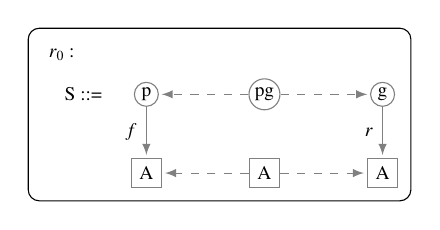
\begin{tikzpicture}[grammar]
	\node[rid] at (\ridX,\ridY) {$r_0:$};
	\draw (\lhsX,0) node[lhs] (lhs) {S ::=};
	
	\draw (0.5,0) node[t] (s1) {p};
	\draw (0.5,-1) node[nont] (s2) {A};
	\draw[edge] (s1) -- (s2) node [vledgeLabel] {$f$};
	%%
	\draw (2,0) node[t] (c1) {pg};
	\draw (2,-1) node[nont] (c2) {A};
	%%
	\draw (3.5,0) node[t] (t1) {g};
	\draw (3.5,-1) node[nont] (t2) {A};
	\draw[edge] (t1) -- (t2) node [vledgeLabel] {$r$};
	%%
	\draw[morph] (c1) -- (s1);
	\draw[morph] (c1) -- (t1);
	\draw[morph] (c2) -- (s2);
	\draw[morph] (c2) -- (t2);
	\end{tikzpicture}
	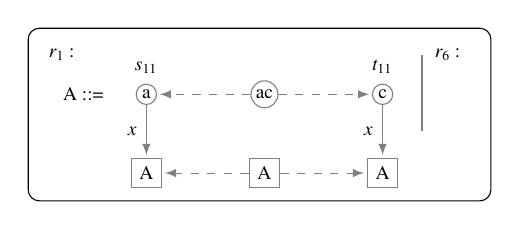
\begin{tikzpicture}[grammar]
	\node[rid] at (\ridX,\ridY) {$r_1:$};
	\draw (\lhsX,0) node[lhs] (lhs) {A ::=};
	
	\draw (0.5,0) node[t, label=90:$s_{11}$] (s1) {a};
	\draw (0.5,-1) node[nont] (s2) {A};
	\draw[edge] (s1) -- (s2) node [vledgeLabel] {$x$};
	%\draw node[uw] at (s1.east) (w-s1) {} [wedge] (s1) -- (w-s1);
	%%
	\draw (2,0) node[t] (c1) {ac};
	\draw (2,-1) node[nont] (c2) {A};
	%%
	\draw (3.5,0) node[t, label=90:$t_{11}$] (t1) {c};
	\draw (3.5,-1) node[nont] (t2) {A};
	\draw[edge] (t1) -- (t2) node [vledgeLabel] {$x$};
	%\draw node[uw] at (t1.north) (w-t1) {} [wedge] (t1) -- (w-t1);
	%%
	\draw[morph] (c1) -- (s1);
	\draw[morph] (c1) -- (t1);
	\draw[morph] (c2) -- (s2);
	\draw[morph] (c2) -- (t2);
	
	%%%%
	\draw[pipe] (4,\pipeBY) -- (4,\pipeUY);
	
	\node[rid] at (4.6,\ridY) {$r_6:$};
	\draw (4.6,0) node[empty] (s3) {$\emptyGraph$};
	\end{tikzpicture}
	
	\noindent
	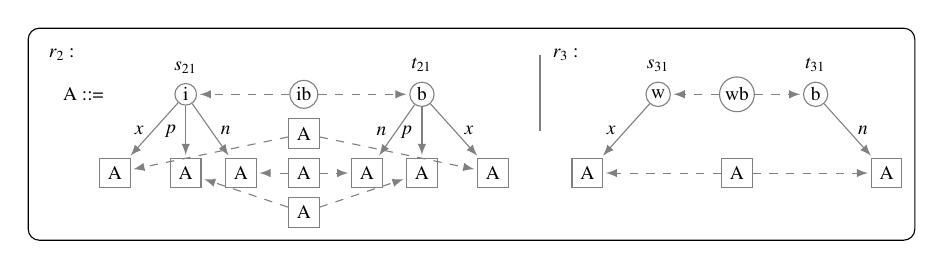
\begin{tikzpicture}[grammar]
	\node[rid] at (\ridX,\ridY) {$r_2:$};
	\draw (\lhsX,0) node[lhs] (lhs) {A ::=};
	
	\draw (1,0) node[t, label=90:$s_{21}$] (s1) {i};
	\draw (0.1,-1) node[nont] (s2) {A};
	\draw (1,-1) node[nont] (s3) {A};
	\draw (1.7,-1) node[nont] (s4) {A};
	\draw[edge] (s1) -- (s2) node [vledgeLabel] {$x$};
	\draw[edge] (s1) -- (s3) node [vledgeLabel] {$p$};
	\draw[edge] (s1) -- (s4) node [vredgeLabel] {$n$};
	%\draw node[uw] at (s1.north) (w-s1) {} [wedge] (s1) -- (w-s1);
	%%
	\draw (2.5,0) node[t] (c1) {ib};
	\draw (2.5,-0.5) node[nont] (c2) {A};
	\draw (2.5,-1) node[nont] (c4) {A};
	\draw (2.5,-1.5) node[nont] (c3) {A};
	%%
	\draw (4,0) node[t, label=90:$t_{21}$] (t1) {b};
	\draw (3.3,-1) node[nont] (t4) {A};
	\draw (4,-1) node[nont] (t3) {A};
	\draw (4.9,-1) node[nont] (t2) {A};
	\draw[edge] (t1) -- (t4) node [vledgeLabel] {$n$};
	\draw[edge] (t1) -- (t3) node [vledgeLabel] {$p$};
	\draw[edge] (t1) -- (t2) node [vredgeLabel] {$x$};
	%\draw node[uw] at (t1.north) (w-t1) {} [wedge] (t1) -- (w-t1);
	%%
	\draw[morph] (c1) -- (s1);
	\draw[morph] (c1) -- (t1);
	\draw[morph] (c2) -- (s2);
	\draw[morph] (c2) -- (t2);
	\draw[morph] (c3) -- (s3);
	\draw[morph] (c3) -- (t3);
	\draw[morph] (c4) -- (s4);
	\draw[morph] (c4) -- (t4);
	
	%%%%
	\draw[pipe] (5.5,\pipeBY) -- (5.5,\pipeUY);
	
	\node[rid] at (6.1,\ridY) {$r_3:$};
	
	\draw (7,0) node[t, label=90:$s_{31}$] (s5) {w};
	\draw (6.1,-1) node[nont] (s6) {A};
	\draw[edge] (s5) -- (s6) node [vledgeLabel] {$x$};
	%\draw node[uw] at (s5.north) (w-s5) {} [wedge] (s5) -- (w-s5);
	%%
	\draw (8,0) node[t] (c5) {wb};
	\draw (8,-1) node[nont] (c6) {A};
	%%
	\draw (9,0) node[t, label=90:$t_{31}$] (t5) {b};
	\draw (9.9,-1) node[nont] (t6) {A};
	\draw[edge] (t5) -- (t6) node [vredgeLabel] {$n$};
	%\draw node[uw] at (t5.north) (w-t5) {} [wedge] (t5) -- (w-t5);
	%%
	\draw[morph] (c5) -- (s5);
	\draw[morph] (c5) -- (t5);
	\draw[morph] (c6) -- (s6);
	\draw[morph] (c6) -- (t6);
	\end{tikzpicture}
	
	\noindent
	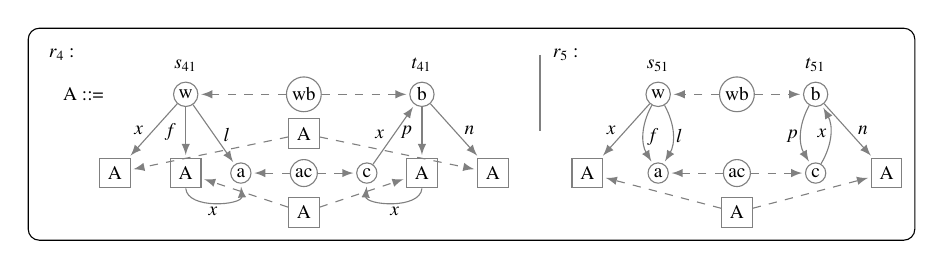
\begin{tikzpicture}[grammar]
	\node[rid] at (\ridX,\ridY) {$r_4:$};
	\draw (\lhsX,0) node[lhs] (lhs) {A ::=};
	
	\draw (1,0) node[t, label=90:$s_{41}$] (s1) {w};
	\draw (0.1,-1) node[nont] (s2) {A};
	\draw (1,-1) node[nont] (s3) {A};
	\draw (1.7,-1) node[t] (s4) {a};
	
	\draw[edge] (s1) -- (s2) node [vledgeLabel] {$x$};
	\draw[edge] (s1) -- (s3) node [vledgeLabel] {$f$};
	\draw[edge] (s3) to [bend right=90] (s4) node [below=10pt, left=5pt] {$x$};
	\draw[edge] (s1) -- (s4) node [vredgeLabel] {$l$};
	%\draw node[uw] at (s1.north) (w-s1) {} [wedge] (s1) -- (w-s1);
	%%
	\draw (2.5,0) node[t] (c1) {wb};
	\draw (2.5,-0.5) node[nont] (c2) {A};
	\draw (2.5,-1) node[t] (c4) {ac};
	\draw (2.5,-1.5) node[nont] (c3) {A};
	%%
	\draw (4,0) node[t, label=90:$t_{41}$] (t1) {b};
	\draw (3.3,-1) node[t] (t4) {c};
	\draw (4,-1) node[nont] (t3) {A};
	\draw (4.9,-1) node[nont] (t2) {A};
	\draw[edge] (t1) -- (t2) node [vredgeLabel] {$n$};
	\draw[edge] (t1) -- (t3) node [vledgeLabel] {$p$};
	\draw[edge] (t3) to [bend left=90] (t4) node [below=10pt, right=5pt] {$x$};
	\draw[edge] (t4) -- (t1) node [vledgeLabel] {$x$};
	%\draw node[uw] at (t1.north) (w-t1) {} [wedge] (t1) -- (w-t1);
	%%
	\draw[morph] (c1) -- (s1);
	\draw[morph] (c1) -- (t1);
	\draw[morph] (c2) -- (s2);
	\draw[morph] (c2) -- (t2);
	\draw[morph] (c3) -- (s3);
	\draw[morph] (c3) -- (t3);
	\draw[morph] (c4) -- (s4);
	\draw[morph] (c4) -- (t4);
	
	%%%%
	\draw[pipe] (5.5,\pipeBY) -- (5.5,\pipeUY);
	
	\node[rid] at (6.1,\ridY) {$r_5:$};
	
	\draw (7,0) node[t, label=90:$s_{51}$] (s5) {w};
	\draw (6.1,-1) node[nont] (s6) {A};
	\draw (7,-1) node[t] (s7) {a};
	\draw[edge] (s5) -- (s6) node [vledgeLabel] {$x$};
	\draw[edge] (s5) to [bend right] (s7) node [vbedgeLabel] {$f$};
	\draw[edge] (s5) to [bend left] (s7) node [above=10pt, right=1pt] {$l$};
	%\draw node[uw] at (s5.north) (w-s5) {} [wedge] (s5) -- (w-s5);
	%%
	\draw (8,0) node[t] (c5) {wb};
	\draw (8,-1.5) node[nont] (c6) {A};
	\draw (8,-1) node[t] (c7) {ac};
	%%
	\draw (9,0) node[t, label=90:$t_{51}$] (t5) {b};
	\draw (9,-1) node[t] (t7) {c};
	\draw (9.9,-1) node[nont] (t6) {A};
	\draw[edge] (t5) -- (t6) node [vredgeLabel] {$n$};
	\draw[edge] (t5) to [bend right] (t7) node [above=10pt, left=1pt] {$p$};
	\draw[edge] (t7) to [bend right] (t5) node [below=5pt] {$x$};
	%\draw node[uw] at (t5.north) (w-t5) {} [wedge] (t5) -- (w-t5);
	%%
	\draw[morph] (c5) -- (s5);
	\draw[morph] (c5) -- (t5);
	\draw[morph] (c6) -- (s6);
	\draw[morph] (c6) -- (t6);
	\draw[morph] (c7) -- (s7);
	\draw[morph] (c7) -- (t7);
	\end{tikzpicture}
		\caption{The depiction of the rules $r_0$ to $r_6$ of the TGG for the transformation between $Pseudocode$ and $Controlflow$ graphs.}
		\label{fig:p2c-tgg}
	\end{figure*}
	
	Notice that, the aforementioned triple graph $TG$ can be generated using the rules of $TGG$ by the following sequence of derivation steps
	$
	\startTG{TGG} \tderivpac{r_0}{}{}{} G_1 \tderivpac{r_2}{}{}{} G_2 \tderivpac{r_6}{}{}{} G_3 \tderivpac{r_1}{}{}{} G_4 \tderivpac{r_6}{}{}{} G_5 \tderivpac{r_1}{}{}{} G_6 \tderivpac{r_4}{}{}{} G_7 \tderivpac{r_1}{}{}{} G_8 \tderivpac{r_6}{}{}{} G_9 \tderivpac{r_1}{}{}{} G_{10} \tderivpac{r_6}{}{}{} TG
	$
	with appropriate $G_i$ for $1 \le i \le 10$.
\end{example}

%TODO: Maybe explain sentential form before
So far, PAC vertices do not have any special influence in the behavior of a derivation step and the set $W$ in a derivation step serves just to tag which vertices are PAC in a sentential form. In particular, the grammar of the Example \ref{ex:pseudocode2controlflow} was not a PAC NCE TGG, so the definition of derivation steps that we posed before would already be enough to define the complete behavior for this grammar.

Nevertheless, PAC vertices play an important role in a PAC NCE TGG, by making it possible for a derivation step to refer to a vertex that is not essentially produced by it, but by another step. This is done via the mechanism of resolution step. The resolution step for the triple graph $G$ to the triple graph $H$ using the resolution partial function $\rho: V_G \pto V_G$, we write $G \tresolv{\rho,\tau} H$, can be described as the removal of the PAC vertices of $G_s$ that are in the domain of the resolution function $\rho$ followed by the redirection of the edges adjacent to these PAC vertices to other vertices of $H_s$, given by the respective image of $\rho$, that are required not to be PAC vertices. The same is performed with the PAC vertices in $G_t$ by $\tau$.

Combining derivation and resolution steps we can define the language of a PAC NCE TGG, what we do in the following.

\begin{definition}
	The language $L(G)$ generated by the PAC NCE TGG $G$ is
	\begin{align*}
	& L(G) = \{ H \text{ is a triple graph over } \Delta \text{ and } \startTG{G}\\
	& \tderivpac{r_0}{s_0,c_0,t_0}{W_0,T_0}{} G_1 \tderivpac{r_1}{s_1,c_1,t_1}{W_1,T_1}{} \dots \\
	& \tderivpac{r_{n-1}}{s_{n-1},c_{n-1},t_{n-1}}{W_{n-1},T_{n-1}}{} G_n^0\\
	& \tresolv{\rho_0,\tau_0} G_n^1 \tresolv{\rho_1,\tau_0} \dots \tresolv{\rho_{n-1},\tau{n-1}} G_n^n
	\end{align*}
	with $\rho_i : m_i(W_i) \to V_{G_n^i}$ and $\tau_i : n_i(T_i) \to V_{G_n^i}$ being the resolution total functions and $m_i : W_i \to V_{G_n^i}$ and $n_i : T_i \to V_{G_n^i}$ the mappings from the PAC vertices generated on the derivation step $i$ to their correspondent vertices in $G_n^i$, for all $0 \le i < n$.
\end{definition}

For the sake of demonstrating how PAC vertices, consider a simplified view of the class diagram metamodel, whose models are encoded via class-diagram graphs. In a such graphs a vertex has either label $c$ or $a$, respectively representing a class or an association, and an edge between an association and a class with label $s$ ($t$) signalizes that the class is the source (target) of the association. In Figure \ref{fig:classdiagram-g}, a class-diagram graph with two classes connected by two associations is depicted. 

\begin{figure}[h]
	\centering
	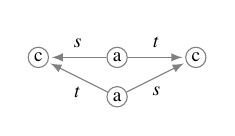
\begin{tikzpicture}[graph]
	\draw (0,0) node[t] (v1) {c};
	\draw (1,0) node[t] (v2) {a};
	\draw (1,-0.5) node[t] (v4) {a};
	\draw (2,0) node[t] (v3) {c};
	\draw[edge] (v2) -- (v1) node [edgeLabel] {$s$};
	\draw[edge] (v2) -- (v3) node [edgeLabel] {$t$};
	\draw[edge] (v4) -- (v3) node [midway, below] {$s$};
	\draw[edge] (v4) -- (v1) node [midway, below] {$t$};
\end{tikzpicture}
	\caption{A class-diagram graph}
	\label{fig:classdiagram-g}
\end{figure}
 
In Figure \ref{fig:classdiagram-gg} we put forward the the rules of the PAC NCE TGG whose language is the set of all class-diagram graphs. This grammar is $GG = (\{K, A, a, c, s, t\}, \{a, c, s, t\}, K, \{r_0, r_1, r_2, r_3\})$ with $\omega_0(c_0) = \{(t,a)\}$, $\omega_2(a_2) = \{(s,c)\}$, $\omega_2(c_2) = \{(s,a),(t,a)\}$, $\omega_1 = \omega_3 = \emptyset$ being the complete characterization of the embedding functions of the respective rules.

\begin{figure}
	\centering
	\noindent
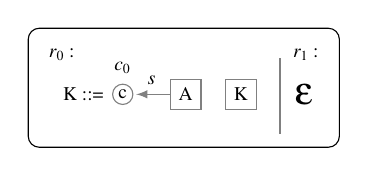
\begin{tikzpicture}[grammar]
	\node[rid] at (\ridX,\ridY) {$r_0:$};
	\draw (\lhsX,0) node[lhs] (lhs) {K ::=};
	
	\draw (0.2,0) node[t, label=90:$c_0$] (v1) {c};
	\draw (1,0) node[nont] (v2) {A};
	\draw (1.7,0) node[nont] (v3) {K};
	\draw[edge] (v2) -- (v1) node [edgeLabel] {$s$};
	
	%The next rule separator
	\draw[pipe] (2.2,-0.5) -- (2.2,\ridY);
	
	\node[rid] at (2.8,\ridY) {$r_1:$};
	\draw (2.5,0) node[empty] (v7) {$\emptyTG$};
\end{tikzpicture}
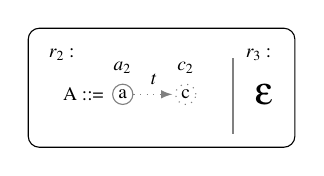
\begin{tikzpicture}[grammar]
\node[rid] at (\ridX,\ridY) {$r_2:$};
\draw (\lhsX,0) node[lhs] (lhs) {A ::=};

\draw (0.2,0) node[t, label=90:$a_2$] (v1) {a};
\draw (1,0) node[pac, label=90:$c_2$] (v2) {c};
\draw[pacedge] (v1) -- (v2) node [edgeLabel] {$t$};

%The next rule separator
\draw[pipe] (1.6,-0.5) -- (1.6,\ridY);

\node[rid] at (2.2,\ridY) {$r_3:$};
\draw (2,0) node[empty] (v7) {$\emptyTG$};
\end{tikzpicture}
	\caption{The depiction of the rules of $GG$}
	\label{fig:classdiagram-gg}
\end{figure}

Below, we demonstrate that the graph from Figure \ref{fig:classdiagram-g} is in $L(GG)$, by means of a sequence of four derivation steps followed by four resolution steps in $GG$.
\begin{align*}
	\startG{GG} \derivpac{r_0}{v_0}{\emptyset}{} &
	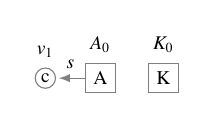
\begin{tikzpicture}[graph]
	\draw (0.5,0) node[t, label=90:$v_1$] (v1) {c};
	\draw (1.2,0) node[nont, label=90:$A_0$] (v2) {A};
	\draw (2,0) node[nont, label=90:$K_0$] (v3) {K};
	\draw[edge] (v2) -- (v1) node [edgeLabel] {$s$};
	\end{tikzpicture}
	\derivpac{r_0}{K_0}{\emptyset}{} &
	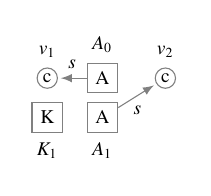
\begin{tikzpicture}[graph]
	\draw (0.5,0) node[t, label=90:$v_1$] (v1) {c};
	\draw (1.2,0) node[nont, label=90:$A_0$] (v2) {A};
	\draw (2,0) node[t, label=90:$v_2$] (v3) {c};
	\draw (1.2,-0.5) node[nont, label=270:$A_1$] (v4) {A};
	\draw (0.5,-0.5) node[nont, label=270:$K_1$] (v5) {K};
	\draw[edge] (v2) -- (v1) node [edgeLabel] {$s$};
	\draw[edge] (v4) -- (v3) node [midway, below] {$s$};
	\end{tikzpicture} \\
	%
	\derivpac{r_1}{K_1}{\emptyset}{} &
	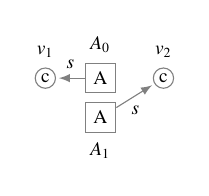
\begin{tikzpicture}[graph]
	\draw (0.5,0) node[t, label=90:$v_1$] (v1) {c};
	\draw (1.2,0) node[nont, label=90:$A_0$] (v2) {A};
	\draw (2,0) node[t, label=90:$v_2$] (v3) {c};
	\draw (1.2,-0.5) node[nont, label=270:$A_1$] (v4) {A};
	\draw[edge] (v2) -- (v1) node [edgeLabel] {$s$};
	\draw[edge] (v4) -- (v3) node [midway, below] {$s$};
	\end{tikzpicture}
	\derivpac{r_2}{A_0}{\{p_0\}}{} &
	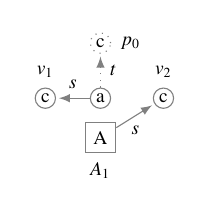
\begin{tikzpicture}[graph]
	\draw (0.5,0) node[t, label=90:$v_1$] (v1) {c};
	\draw (1.2,0) node[t] (v2) {a};
	\draw (1.2,0.7) node[pac, label=0:$p_0$] (v5) {c};
	\draw (2,0) node[t, label=90:$v_2$] (v3) {c};
	\draw (1.2,-0.5) node[nont, label=270:$A_1$] (v4) {A};
	\draw[edge] (v2) -- (v1) node [edgeLabel] {$s$};
	\draw[pacedge] (v2) -- (v5) node [vredgeLabel] {$t$};
	\draw[edge] (v4) -- (v3) node [midway, below] {$s$};
	\end{tikzpicture}
\end{align*}
\begin{align*}
	\derivpac{r_2}{A_1}{\{p_1\}}{} &
	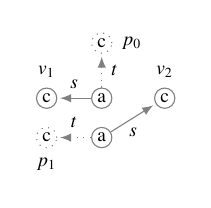
\begin{tikzpicture}[graph]
	\draw (0.5,0) node[t, label=90:$v_1$] (v1) {c};
	\draw (1.2,0) node[t] (v2) {a};
	\draw (1.2,0.7) node[pac, label=0:$p_0$] (v5) {c};
	\draw (2,0) node[t, label=90:$v_2$] (v3) {c};
	\draw (1.2,-0.5) node[t] (v4) {a};
	\draw (0.5,-0.5) node[pac, label=270:$p_1$] (v6) {c};
	\draw[edge] (v2) -- (v1) node [edgeLabel] {$s$};
	\draw[pacedge] (v2) -- (v5) node [vredgeLabel] {$t$};
	\draw[edge] (v4) -- (v3) node [midway, below] {$s$};
	\draw[pacedge] (v4) -- (v6) node [edgeLabel] {$t$};
	\end{tikzpicture}
	\;\;\; \resolvn{\emptyset}{}{3} \;\;\; &
	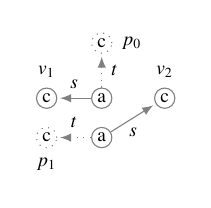
\begin{tikzpicture}[graph]
	\draw (0.5,0) node[t, label=90:$v_1$] (v1) {c};
	\draw (1.2,0) node[t] (v2) {a};
	\draw (1.2,0.7) node[pac, label=0:$p_0$] (v5) {c};
	\draw (2,0) node[t, label=90:$v_2$] (v3) {c};
	\draw (1.2,-0.5) node[t] (v4) {a};
	\draw (0.5,-0.5) node[pac, label=270:$p_1$] (v6) {c};
	\draw[edge] (v2) -- (v1) node [edgeLabel] {$s$};
	\draw[pacedge] (v2) -- (v5) node [vredgeLabel] {$t$};
	\draw[edge] (v4) -- (v3) node [midway, below] {$s$};
	\draw[pacedge] (v4) -- (v6) node [edgeLabel] {$t$};
	\end{tikzpicture} \\
	%
	\;\;\; \resolv{\{p_0 \mapsto v_2\}}{} &
	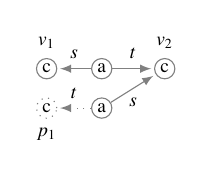
\begin{tikzpicture}[graph]
	\draw (0.5,0) node[t, label=90:$v_1$] (v1) {c};
	\draw (1.2,0) node[t] (v2) {a};
	\draw (2,0) node[t, label=90:$v_2$] (v3) {c};
	\draw (1.2,-0.5) node[t] (v4) {a};
	\draw (0.5,-0.5) node[pac, label=270:$p_1$] (v6) {c};
	\draw[edge] (v2) -- (v1) node [edgeLabel] {$s$};
	\draw[edge] (v2) -- (v3) node [edgeLabel] {$t$};
	\draw[edge] (v4) -- (v3) node [midway, below] {$s$};
	\draw[pacedge] (v4) -- (v6) node [edgeLabel] {$t$};
	\end{tikzpicture}
	\resolv{\{p_1 \mapsto v_1\}}{} \;\;\; &
	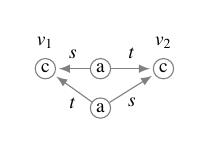
\begin{tikzpicture}[graph]
	\draw (0.5,0) node[t, label=90:$v_1$] (v1) {c};
	\draw (1.2,0) node[t] (v2) {a};
	\draw (2,0) node[t, label=90:$v_2$] (v3) {c};
	\draw (1.2,-0.5) node[t] (v4) {a};
	\draw[edge] (v2) -- (v1) node [edgeLabel] {$s$};
	\draw[edge] (v2) -- (v3) node [edgeLabel] {$t$};
	\draw[edge] (v4) -- (v3) node [midway, below] {$s$};
	\draw[edge] (v4) -- (v1) node [midway, below] {$t$};
	\end{tikzpicture}
\end{align*}

%TODO: Maybe need to explain descendant and precedent vertices
In this sequence of derivation and resolution steps, the rule $r_2$ creates, through two applications, two PAC vertices $p_0$ and $p_1$, which are then removed and have their adjacent vertices moved to the vertices $v_2$ and $v_1$, respectively, through the last two resolution steps. The resolution steps have thus the power of connecting vertices that could not be connected otherwise, because in a NCE TGG without PAC, a vertex in any sentential form can only be either connected to vertices that stem from the same rule application or to neighbors of its precedent vertex.

\section{\uppercase{Model Transformation with PAC NCE TGG}}

\noindent

\section{\uppercase{Evaluation}}

\noindent In order to evaluate the usability of the proposed BNCE TGG formalism, we compare the number of rules and elements (vertices, edges, and mappings) we needed to describe some model transformations in BNCE TGG and in standard TGG without application conditions. Table \ref{tab:formalism-eval} presents these results.

In the case of $Pseudocode2Controlflow$, our proposed approach shows a clear advantage against the standard TGG formalism. We judge that similarly to what happens to programming languages, this advantage stems from the very nested structure of $Pseudocode$ and $Controlflow$ graphs. That is, for instance, in rule the $r_2$ of this TGG (see Example \ref{ex:pseudocode2controlflow}), a node in a positive branch of an $if$-labeled vertex is never connected with a node in the negative branch. This disjunctive aspect allows every branch to be defined in the rule (as well as effectively parsed) independently of the other branch. This characteristic makes it possible for BNCE TGG rules to be defined in a very straightforward manner and reduces the total number of elements necessary.

\begin{table*}
	\setlength{\tabcolsep}{10pt}
	\centering
	\begin{tabular}{l r r r r }
		\hline
		& \multicolumn{2}{c}{Standard TGG} & \multicolumn{2}{c}{BNCE TGG}\\
		Transformation 			& Rules & Elements 	& Rules & Elements\\
		\hline
		Pseudocode2Controlflow	& 45			& 1061	& \textbf{7}	& \textbf{185} \\
		BTree2XBTree			& \textbf{4}	& \textbf{50}	& 5		& 80 \\
		Star2Wheel				& -				& -		& \textbf{6} 	& \textbf{89} \\
		Class2Database			& \textbf{6}	& \textbf{98}	& 	&  \\
		Statemachine2Petrinet	& 	& 	& 	&  \\
		\hline
	\end{tabular}
	\caption{Results of the usability evaluation of the BNCE TGG formalism in comparison with the standard TGG for the model transformation problem}
	\label{tab:formalism-eval}
\end{table*}

In addition to that, the use of non-terminal symbols gives BNCE TGG the power to represent abstract concepts very easily. For example, whereas the rule $r_1$ encodes, using only few elements, that after each $action$ comes any statement $A$, which can be another $action$, an $if$, a $while$ or nothing (an empty graph), in the standard TGG without application condition or any special inheritance treatment, we need to write a different rule for each of these cases. For the whole grammar, we need to consider all combinations of $actions$, $ifs$ and $whiles$ in all rules, what causes the great number of rules and elements.

The $Star2Wheel$ transformation consists of transforming star graphs, which are complete bipartite graphs $K_{1,k}$--- where the partitions are named center and border--- to wheel graphs, that can be constructed from star graphs by adding edges between border vertices to form a minimal cycle. We could not describe this transformation in standard TGG, especially because of the rules' monotonicity (see Definition \ref{def:stgg}). That is, we missed the possibility to erase edges in a rule, feature that we do have in the semantics of BNCE TGG through the embedding mechanism.

\section{\uppercase{Conclusion}}

\noindent


\vfill
\bibliographystyle{apalike}
{\small
\bibliography{bibliography}}

\vfill
\end{document}

